\begin{figure}[ht]
  \centering
  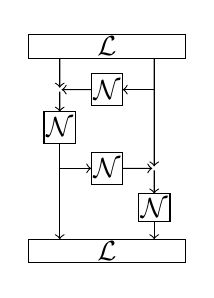
\begin{tikzpicture}[scale=0.4]
    % Drawing the S- and L- Boxes from bottom to top
    \draw
    (-2.50, +0.00) rectangle (+2.50, +0.75) node[pos=0.5]{$\mathcal{L}$}
    (+1.00, +1.30) rectangle (+2.00, +2.20) node[pos=0.5]{$\mathcal{N}$}
    (-0.50, +2.50) rectangle (+0.50, +3.50) node[pos=0.5]{$\mathcal{N}$}
    (+1.50, +3.00) node[inner sep=0] (mult_bottom) {$\fmult$}
    % Top part
    (-2.00, +3.80) rectangle (-1.00, +4.80) node[pos=0.5]{$\mathcal{N}$}
    (-0.50, +5.00) rectangle (+0.50, +6.00) node[pos=0.5]{$\mathcal{N}$}
    (-1.50, +5.50) node[inner sep=0] (mult_top) {$\fmult$}
    (-2.50, +6.50) rectangle (+2.50, +7.25) node[pos=0.5]{$\mathcal{L}$}
    ;
    % Arrows from bottom to top
    \draw[->] (+1.50, +1.30) -- (+1.50, +0.75) ;
    \draw[->] (mult_bottom)  -- (+1.50, +2.20) ;
    \draw[->] (+0.50, +3.00) -- (mult_bottom)  ;
    \draw[->] (-1.50, +3.80) -- (-1.50, +0.75) ;
    \draw[->] (-1.50, +3.00) -- (-0.50, +3.00) ;
    \draw[->] (mult_top)     -- (-1.50, +4.80) ;
    \draw[->] (-0.50, +5.50) -- (mult_top)     ;
    \draw[->] (+1.50, +5.50) -- (+0.50, +5.50) ;
    \draw[->] (+1.50, +6.50) -- (mult_bottom)  ;
    \draw[->] (-1.50, +6.50) -- (mult_top)     ;
  \end{tikzpicture}  
  \TabDef{simplified}{A simplified decomposition of $\pi$. Linear
    (resp. non linear) functions are denoted $\mathcal{L}$
    (resp. $\mathcal{N}$) and $\fmult$ is a finite field
    multiplication.}
\end{figure}